\documentclass[../structural_economics_book.tex]{subfiles}
\begin{document}
\ifSubfilesClassLoaded{\setcounter{chapter}{12}}{}
\chapter{How Networks Evolve}\label{ch:13}
\chaptersubtitle{The Dynamics of Structural Change}
\begin{quote}
\textit{``La internacionalizaci\'{o}n de la econom\'{i}a tiene como contrapartida la desintegraci\'{o}n nacional: al mismo tiempo que se van creando v\'{i}nculos intensos entre los n\'{u}cleos din\'{a}micos de los pa\'{i}ses subdesarrollados y el sistema econ\'{o}mico internacional, se van desarticulando los v\'{i}nculos entre esos n\'{u}cleos y el resto de la econom\'{i}a nacional.''}\\[0.3em]
\textnormal{[``The internationalization of the economy has as its counterpart national disintegration: at the same time that intense links are created between the dynamic nuclei of underdeveloped countries and the international economic system, the links between those nuclei and the rest of the national economy are dismantled.'']}\\
\hfill --- Osvaldo Sunkel, ``Capitalismo transnacional y desintegraci\'{o}n nacional'' (1971)
\end{quote}

\vspace{1em}

Parts~I--III treated the weight matrices $(W^U, W^P, W^I)$ as given. We asked: given the network, what is the equilibrium allocation, the power structure, the preference formation? But the networks themselves change. Trade routes open and close. Firms enter and exit. Social media platforms rewire who talks to whom. The question of Part~IV is: \textit{how does $W$ evolve, and what determines whether it evolves toward integration or fragmentation?}

This chapter develops the general theory of network evolution. The central result: $W$ changes through three mechanisms --- edge creation (new links form), edge destruction (existing links break), and edge reweighting (the strength of existing links changes). Each mechanism is governed by the current state of the economy: the allocation, the returns, and the preferences. This creates a \textbf{co-evolution}: $W$ shapes $(\x^*, \boldsymbol{\theta}^*)$ (the static model of Parts~I--III), and $(\x^*, \boldsymbol{\theta}^*)$ shapes the next period's $W$. The steady state of the co-evolutionary system is the \textbf{structural equilibrium}: a weight matrix that reproduces itself through the allocation and preferences it generates.


%% =====================================================================
\section{Three Mechanisms of Network Change}
\label{ch13:sec:mechanisms}
%% =====================================================================

\subsection{Edge Creation}

New edges form when agents establish new connections. In $W^P$: a firm opens a supply contract with a new input provider. In $W^U$: a migrant forms a friendship in a new city. In $W^I$: a student enrolls in a university and begins receiving signals from a new reference group.

\begin{definition}[Edge Creation Process]\label{ch13:def:creation}
The probability that a new edge $(i, j)$ forms in period $t+1$ depends on three factors:
\begin{equation}\label{ch13:eq:creation}
\Pr(\Delta W_{ij,t+1} > 0 \mid W_t) = p_0 + p_1 \cdot \underbrace{d(i, j; W_t)}_{\text{network distance}} + p_2 \cdot \underbrace{s(i, j; \x_t^*)}_{\text{surplus from connection}} + p_3 \cdot \underbrace{q(i, j; W^I_t)}_{\text{information about } j},
\end{equation}
where:
\begin{itemize}
\item $d(i, j; W_t)$: \textbf{proximity in the existing network.} Agents form links more easily with friends of friends (triadic closure). The probability of connecting to $j$ increases if $i$ and $j$ share a neighbor. This is the relatedness mechanism: new connections form near existing ones.
\item $s(i, j; \x_t^*)$: \textbf{expected surplus from the connection.} $i$ connects to $j$ if the connection generates value --- a profitable trade, a useful signal, a beneficial relationship. The surplus depends on the current allocation (which determines prices and returns).
\item $q(i, j; W^I_t)$: \textbf{information.} $i$ can only form a link with $j$ if $i$ \textit{knows about} $j$. Knowledge of potential partners is filtered through $W^I$: you connect to people you have heard of, which are people in your information network's reach.
\end{itemize}
\end{definition}

\begin{intuition}[Why proximity dominates]
The three factors create a strong path dependence. New edges form near existing edges (proximity), where the surplus is predictable (information), and where the connection can be sustained (surplus). This means $W_{t+1}$ is similar to $W_t$: the network evolves gradually, not by random rewiring. The principle of relatedness (Hidalgo et al., 2007) --- the empirical law that regions diversify into activities related to their existing activities --- is a consequence of this proximity mechanism applied to $W^P$.
\end{intuition}


\subsection{Edge Destruction}

Existing edges break when the surplus from maintaining them turns negative, or when an exogenous shock disrupts the connection.

\begin{definition}[Edge Destruction Process]\label{ch13:def:destruction}
An existing edge $(i, j)$ is destroyed in period $t+1$ with probability:
\begin{equation}\label{ch13:eq:destruction}
\Pr(W_{ij,t+1} = 0 \mid W_{ij,t} > 0) = \delta_0 + \delta_1 \cdot \underbrace{\max(0, -s(i, j; \x_t^*))}_{\text{negative surplus}} + \delta_2 \cdot \underbrace{\sigma_{ij,t}}_{\text{exogenous shock}},
\end{equation}
where $\delta_0$ is the baseline destruction rate (natural turnover), $s < 0$ means the link is unprofitable, and $\sigma_{ij,t}$ is an exogenous shock (a crisis, a policy change, a natural disaster that severs a trade route).
\end{definition}

\begin{example}[Bolivia's Gas Nationalization as Edge Destruction and Creation]\label{ch13:ex:gas}
Bolivia's nationalization of gas in 2006 was a simultaneous edge destruction and edge creation event in $W^P$:

\textbf{Destruction:} The edges from domestic gas production to foreign MNC headquarters ($W^P_{\text{Bolivia, MNC}}$) were weakened. Foreign companies lost operational control. The profits channel (surplus flowing from Bolivia to MNC shareholders) was partially severed.

\textbf{Creation:} New edges from gas production to the domestic treasury ($W^P_{\text{gas, treasury}}$) were strengthened. Gas revenues began flowing through domestic fiscal channels to domestic social programs.

\textbf{Net effect on $\Gamma$:} Ambiguous. The nationalization increased some within-country linkages (gas revenue to social spending) but did not create production linkages between the gas sector and the traditional economy. The upper-left block of $W^P$ (gas/government) became brighter internally, but the cross-block entries (gas to traditional) remained dark. $\Gamma$ may have increased slightly (more domestic fiscal links) without fundamentally changing the block-diagonal structure.
\end{example}


\subsection{Edge Reweighting}

The strength of existing edges changes continuously as the economic environment evolves.

\begin{definition}[Edge Reweighting]\label{ch13:def:reweighting}
The weight of an existing edge evolves according to:
\begin{equation}\label{ch13:eq:reweighting}
W_{ij,t+1} = W_{ij,t} + \eta \cdot \frac{\partial s(i,j)}{\partial W_{ij}} + \nu_{ij,t},
\end{equation}
where $\eta > 0$ governs the speed of adjustment and $\nu_{ij,t}$ is noise. Profitable connections strengthen ($\partial s / \partial W > 0$); unprofitable connections weaken.
\end{definition}


%% =====================================================================
\section{The General Network Evolution Equation}
\label{ch13:sec:evolution}
%% =====================================================================

Combining creation, destruction, and reweighting, the network evolves according to:

\begin{definition}[Network Evolution Equation]\label{ch13:def:evolution}
\begin{equation}\label{ch13:eq:evolution}
W_{t+1} = \underbrace{(1 - D_t) \circ W_t}_{\text{surviving edges}} + \underbrace{C_t \circ \tilde{W}_{t+1}}_{\text{new edges}} + \underbrace{\eta \cdot S_t}_{\text{reweighting}},
\end{equation}
where $\circ$ is the Hadamard (element-wise) product, $D_t$ is the $N \times N$ destruction probability matrix, $C_t$ is the creation probability matrix, $\tilde{W}_{t+1}$ is the weight assigned to newly created edges, and $S_t = [\partial s(i,j)/\partial W_{ij}]$ is the surplus gradient matrix.
\end{definition}

\begin{theorem}[The Co-Evolutionary System]\label{ch13:thm:coevolution}
The complete structural economics model is a co-evolutionary system in $(W_t, \boldsymbol{\theta}_t)$:
\begin{align}
\boldsymbol{\theta}_{t+1} &= \Phi(\boldsymbol{\theta}_t; W_t) \quad \text{(formation equation, Chapter~10)}, \label{ch13:eq:coev_theta} \\
W_{t+1} &= \Psi(W_t; \x^*(\boldsymbol{\theta}_t, W_t)) \quad \text{(network evolution equation)}, \label{ch13:eq:coev_W}
\end{align}
where $\x^*(\boldsymbol{\theta}_t, W_t)$ is the bargaining equilibrium at period $t$.

The fast variable is $\x^*$ (clears within a period). The medium variable is $\boldsymbol{\theta}$ (adjusts across generations). The slow variable is $W$ (evolves over decades or centuries). Three timescales, nested.
\end{theorem}

\begin{intuition}[Three timescales]
Markets clear in months. Preferences form in generations. Structures evolve over centuries. This ordering is what makes the analysis tractable: at any given timescale, the slower variables are approximately constant and the faster variables are in approximate equilibrium.

When we analyzed the bargaining equilibrium (Chapters~6--7), we held $W$ and $\boldsymbol{\theta}$ fixed --- both are slow relative to market clearing. When we analyzed the formation model (Chapters~9--10), we held $W$ fixed --- it is slow relative to preference formation. Now we let $W$ move, completing the picture.
\end{intuition}


%% =====================================================================
\section{Structural Equilibrium}
\label{ch13:sec:structural_eq}
%% =====================================================================

\subsection{Definition}

\begin{definition}[Structural Equilibrium]\label{ch13:def:structural_eq}
A \textbf{structural equilibrium} is a triple $(W^*, \boldsymbol{\theta}^*, \x^*)$ satisfying:
\begin{enumerate}
\item $\x^* = h(\boldsymbol{\pi}(W^*), \boldsymbol{\theta}^*, \boldsymbol{\omega})$ (bargaining equilibrium),
\item $\boldsymbol{\theta}^* = \Phi(\boldsymbol{\theta}^*; W^*)$ (formation steady state),
\item $W^* = \Psi(W^*; \x^*)$ (network steady state).
\end{enumerate}
All three equations are simultaneously satisfied. The weight matrix produces the allocation and preferences that reproduce the weight matrix.
\end{definition}

\begin{theorem}[Existence of Structural Equilibrium]\label{ch13:thm:existence}
Under regularity conditions (continuous $\Phi$, $\Psi$, $h$; compact domains; bounded weights), at least one structural equilibrium exists.
\end{theorem}

\begin{proof}[Proof sketch]
Define the composite map $\Xi: (W, \boldsymbol{\theta}) \mapsto (\Psi(W; h(\boldsymbol{\pi}(W), \Phi(\boldsymbol{\theta}; W), \boldsymbol{\omega})), \Phi(\boldsymbol{\theta}; W))$. On the compact convex product space $\mathcal{W} \times \Theta$ (where $\mathcal{W}$ is the space of row-stochastic matrices and $\Theta$ a bounded preference domain), $\Xi$ is continuous. Brouwer's fixed-point theorem guarantees existence.
\end{proof}


\subsection{Multiple Structural Equilibria}

\begin{proposition}[Multiplicity]\label{ch13:prop:multiplicity}
The co-evolutionary system generically admits multiple structural equilibria. Two important types:

\textbf{The integrated equilibrium.} $W^*$ has large $\Gamma$ (well-connected), $\boldsymbol{\theta}^*$ is approximately uniform (homogeneous preferences), $\x^*$ is close to equal division. Cross-block edges are sustained by positive surplus. This equilibrium is self-reinforcing: the connected structure produces high returns for all agents, which sustains the preferences that support the connections, which maintains the structure.

\textbf{The fragmented equilibrium.} $W^*$ is approximately block-diagonal (small $\Gamma$), $\boldsymbol{\theta}^*$ is stratified (different preferences per block), $\x^*$ is highly unequal. Cross-block edges do not form because the surplus is too low (the traditional block's agents cannot afford the investment needed to link to the modern block). This equilibrium is also self-reinforcing: the disconnected structure produces low returns in the traditional block, which forms low aspirations, which prevents investment in cross-block links, which maintains disconnection.
\end{proposition}

\begin{example}[Two Structural Equilibria for Bolivia]\label{ch13:ex:bolivia_two}
$N = 6$: Gas block (agents 1--2), Urban block (agents 3--4), Rural block (agents 5--6). Parameters: $\rho = 0.85$, $\mu = 0.2$, $\eta = 0.05$, $p_1 = 0.3$ (proximity dominates edge creation).

\textbf{Equilibrium A (Fragmented):}
\begin{equation}
W^*_A = \begin{pmatrix}
0.4 & 0.4 & 0.02 & 0.02 & 0.01 & 0.01 \\
0.4 & 0.4 & 0.02 & 0.02 & 0.01 & 0.01 \\
0.02 & 0.02 & 0.35 & 0.35 & 0.05 & 0.05 \\
0.02 & 0.02 & 0.35 & 0.35 & 0.05 & 0.05 \\
0.01 & 0.01 & 0.05 & 0.05 & 0.40 & 0.40 \\
0.01 & 0.01 & 0.05 & 0.05 & 0.40 & 0.40
\end{pmatrix}.
\end{equation}

$\Gamma_A \approx 0.06$. $\boldsymbol{\theta}^* \approx (1.12, 1.12, 1.01, 1.01, 0.91, 0.91)$. $\boldsymbol{\pi} \approx (0.22, 0.22, 0.17, 0.17, 0.11, 0.11)$. Max allocation gap: 38\%.

\textbf{Equilibrium B (Integrated):}
\begin{equation}
W^*_B = \begin{pmatrix}
0.25 & 0.20 & 0.12 & 0.12 & 0.08 & 0.08 \\
0.20 & 0.25 & 0.12 & 0.12 & 0.08 & 0.08 \\
0.12 & 0.12 & 0.20 & 0.18 & 0.10 & 0.10 \\
0.12 & 0.12 & 0.18 & 0.20 & 0.10 & 0.10 \\
0.08 & 0.08 & 0.10 & 0.10 & 0.22 & 0.22 \\
0.08 & 0.08 & 0.10 & 0.10 & 0.22 & 0.22
\end{pmatrix}.
\end{equation}

$\Gamma_B \approx 0.35$. $\boldsymbol{\theta}^* \approx (1.06, 1.06, 1.02, 1.02, 0.97, 0.97)$. $\boldsymbol{\pi} \approx (0.19, 0.19, 0.17, 0.17, 0.14, 0.14)$. Max allocation gap: 12\%.

Same economy, same parameters. Two self-reinforcing structures. Which obtains depends on history.
\end{example}

\begin{vizpanel}{Two structural equilibria: fragmented and integrated}
\begin{center}
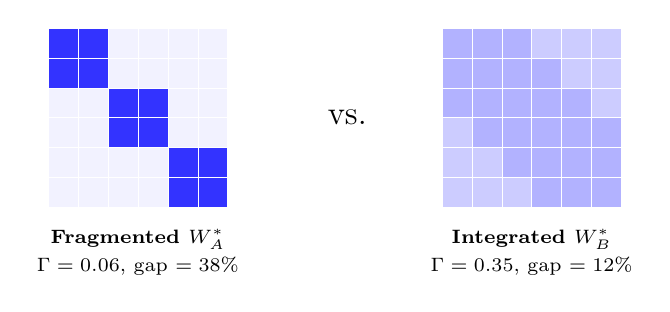
\begin{tikzpicture}[scale=1]
\def\N{6}
\def\s{0.38}

%% Fragmented
\foreach \i in {1,...,\N} {
  \foreach \j in {1,...,\N} {
    \pgfmathparse{
      (\i<=2 && \j<=2) ? 80 :
      (\i>=3 && \i<=4 && \j>=3 && \j<=4) ? 70 :
      (\i>=5 && \j>=5) ? 80 :
      5
    }
    \edef\bp{\pgfmathresult}
    \fill[blue!\bp, draw=white, line width=0.1pt]
      ({(\j-1)*\s}, {(\N-\i)*\s}) rectangle +(\s,\s);
  }
}
\node[below, font=\scriptsize\bfseries] at ({3*\s}, -0.15) {Fragmented $W^*_A$};
\node[below, font=\scriptsize] at ({3*\s}, -0.5) {$\Gamma = 0.06$, gap $= 38\%$};

\node[font=\large] at (3.8, 1.14) {vs.};

%% Integrated
\begin{scope}[xshift=5cm]
\foreach \i in {1,...,\N} {
  \foreach \j in {1,...,\N} {
    \pgfmathparse{
      (\i<=2 && \j<=2) ? 60 :
      (\i>=3 && \i<=4 && \j>=3 && \j<=4) ? 50 :
      (\i>=5 && \j>=5) ? 55 :
      (abs(\i-\j)<=2) ? 30 :
      20
    }
    \edef\bp{\pgfmathresult}
    \fill[blue!\bp, draw=white, line width=0.1pt]
      ({(\j-1)*\s}, {(\N-\i)*\s}) rectangle +(\s,\s);
  }
}
\node[below, font=\scriptsize\bfseries] at ({3*\s}, -0.15) {Integrated $W^*_B$};
\node[below, font=\scriptsize] at ({3*\s}, -0.5) {$\Gamma = 0.35$, gap $= 12\%$};
\end{scope}
\end{tikzpicture}
\end{center}
\vspace{-0.5em}
\small Same economy, same parameters, same production functions. Left: the fragmented equilibrium --- three bright blocks, dark cross-block. Right: the integrated equilibrium --- blocks still visible but cross-block entries are bright. Both are self-reinforcing. Which one you get depends on where you start.
\end{vizpanel}


%% =====================================================================
\section{The Principle of Relatedness}
\label{ch13:sec:relatedness}
%% =====================================================================

The edge creation process (Definition~\ref{ch13:def:creation}) implies that new edges form near existing edges. This has a powerful consequence: the network's evolution is path-dependent.

\begin{theorem}[Path Dependence of Network Evolution]\label{ch13:thm:path_dependence}
If edge creation is dominated by proximity ($p_1 \gg p_2, p_3$ in~\eqref{ch13:eq:creation}), then:
\begin{enumerate}
\item $W_{t+1}$ is structurally similar to $W_t$: new edges connect agents who are already close in the network.
\item The spectral gap $\Gamma_t$ changes slowly: $|\Gamma_{t+1} - \Gamma_t| \leq C \cdot \|W_{t+1} - W_t\|$.
\item Block-diagonal structures are absorbing: if $W_t$ is approximately block-diagonal, new edges form within blocks (high proximity) rather than between blocks (low proximity), reinforcing the block-diagonal structure.
\item Escaping a block-diagonal structure requires either (a) a large exogenous shock that creates cross-block edges, or (b) deliberate policy that overrides the proximity mechanism.
\end{enumerate}
\end{theorem}

\begin{proof}[Proof sketch]
(1) follows directly from the proximity term dominating: $\Pr(\text{new edge}) \propto d(i,j; W_t)$, which is high for agents already close in $W_t$. (2) follows from matrix perturbation theory (Appendix 3A): small changes in $W$ produce small changes in eigenvalues. (3): in a block-diagonal $W_t$, within-block distances are small and cross-block distances are large. Edge creation favors short distances, so new edges form within blocks. (4): escaping requires adding edges with low proximity, which the proximity mechanism suppresses.
\end{proof}

\begin{prebisch}[The principle of relatedness as structural lock-in]
The principle of relatedness (Hidalgo et al., 2007; Hidalgo, 2021) states that the probability a region enters a new economic activity increases with the number of related activities already present. In the product space, countries diversify into products near their current exports, not into distant products.

This IS Theorem~\ref{ch13:thm:path_dependence} applied to $W^P$. The production network evolves through proximity-dominated edge creation: you can produce what is ``near'' what you already produce. Bolivia produces gas (a product on the periphery of the product space, few connections to other products). The nearest products are other extractive commodities (mining, basic chemicals). The distant products are machinery, electronics, pharmaceuticals --- the dense core of the product space where $\Gamma$ is high.

The principle of relatedness is simultaneously the mechanism of industrial deepening (in the center: you diversify into related products, building an ever-denser $W^P$) and the mechanism of structural lock-in (in the periphery: you diversify into related commodities, staying on the sparse periphery of $W^P$). The same mechanism produces integration in the center and fragmentation in the periphery. This is not a paradox --- it is a property of the proximity kernel: diversification follows edges, and the edge structure is dense in the core and sparse on the periphery.
\end{prebisch}


%% =====================================================================
\section{Integration and Disintegration}
\label{ch13:sec:integration}
%% =====================================================================

\subsection{When Does $\Gamma$ Increase?}

\begin{proposition}[Conditions for Structural Integration]\label{ch13:prop:integration}
$\Gamma_{t+1} > \Gamma_t$ (the spectral gap increases --- the economy becomes more integrated) if and only if the net effect of edge creation, destruction, and reweighting increases the relative weight of cross-block edges compared to within-block edges.

Sufficient conditions:
\begin{enumerate}
\item \textbf{Cross-block surplus is positive}: $s(i, j) > 0$ for $i \in$ block $b$, $j \in$ block $b'$ ($b \neq b'$). Trade between blocks is profitable.
\item \textbf{Information reaches across blocks}: $q(i, j; W^I) > 0$ for cross-block pairs. Agents in block $b$ know about opportunities in block $b'$.
\item \textbf{Proximity barriers are overcome}: either by exogenous shocks that create cross-block edges (a road, a migration wave, a new trade route), or by policy that subsidizes cross-block links.
\end{enumerate}
\end{proposition}

\subsection{When Does $\Gamma$ Decrease?}

\begin{proposition}[Conditions for Structural Disintegration]\label{ch13:prop:disintegration}
$\Gamma_{t+1} < \Gamma_t$ (the spectral gap decreases --- the economy fragments) when:
\begin{enumerate}
\item \textbf{Cross-block edges are destroyed faster than created}: an external shock severs trade routes, a policy closes borders, a financial crisis disrupts supply chains.
\item \textbf{Within-block edges strengthen at the expense of cross-block edges}: agents retrench to familiar partners under uncertainty.
\item \textbf{Selective integration}: some agents in each block form cross-border links (the elite), while the remaining agents lose cross-block links. The average $\Gamma$ may be unchanged, but the domestic $\Gamma$ falls.
\end{enumerate}
\end{proposition}

\begin{keyinsight}
Condition~3 is Sunkel's thesis: \textit{transnational integration and national disintegration are the same process.} When the gas executive in La Paz connects to the global commodity market ($W^P_{\text{executive, global}}$ strengthens), his connection to the quinoa farmer weakens ($W^P_{\text{executive, farmer}}$ weakens --- his supply chains are now global, not domestic). The global $\Gamma$ increases (more connected world economy). The domestic $\Gamma$ decreases (more fragmented national economy). The same edge creation (gas executive $\to$ global market) is simultaneously integration at one scale and disintegration at another.
\end{keyinsight}


\subsection{A Phase Diagram}

\begin{proposition}[Phase Diagram for $\Gamma$]\label{ch13:prop:phase}
In the co-evolutionary system, the dynamics of $\Gamma_t$ can be approximated by:
\begin{equation}\label{ch13:eq:gamma_dynamics}
\Gamma_{t+1} - \Gamma_t \approx \underbrace{\eta_c \cdot s_{\text{cross}}(W_t, \x^*_t)}_{\text{integration force}} - \underbrace{\eta_d \cdot \delta_{\text{cross}}(W_t)}_{\text{fragmentation force}} - \underbrace{\eta_p \cdot (p_1 - p_1^*)}_{\text{proximity bias}},
\end{equation}
where $s_{\text{cross}}$ is the average cross-block surplus, $\delta_{\text{cross}}$ is the cross-block destruction rate, and $p_1 - p_1^*$ measures how much edge creation is proximity-biased relative to the threshold $p_1^*$ that would maintain the current $\Gamma$.

\textbf{Three regimes}:
\begin{enumerate}
\item \textbf{Integration}: $s_{\text{cross}} > 0$ and $\delta_{\text{cross}}$ is low. The economy moves toward the integrated equilibrium. $\Gamma \uparrow$.
\item \textbf{Fragmentation}: $s_{\text{cross}} < 0$ or $\delta_{\text{cross}}$ is high. The economy moves toward the fragmented equilibrium. $\Gamma \downarrow$.
\item \textbf{Lock-in}: $s_{\text{cross}} \approx 0$ and proximity dominates. $\Gamma$ is approximately constant. The economy is trapped in its current structural configuration.
\end{enumerate}
\end{proposition}

\begin{vizpanel}{Phase diagram: integration vs.\ fragmentation forces}
\begin{center}
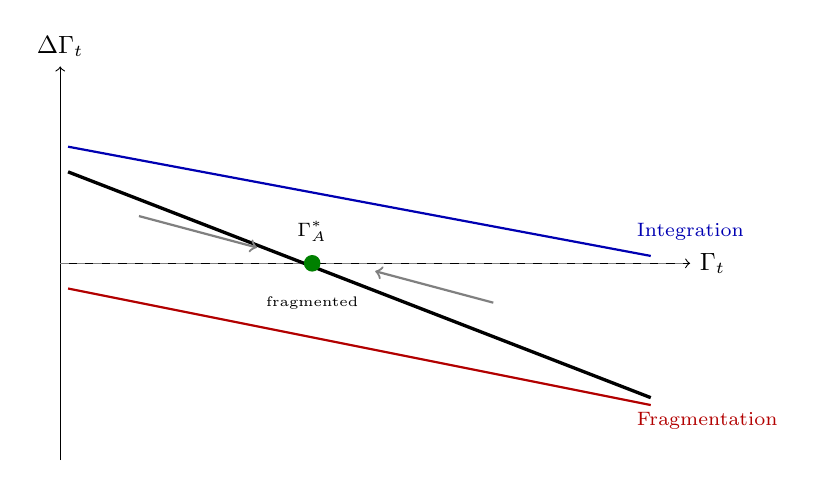
\begin{tikzpicture}[scale=1]
%% Axes
\draw[->] (0,0) -- (8,0) node[right, font=\small] {$\Gamma_t$};
\draw[->] (0,-2.5) -- (0,2.5) node[above, font=\small] {$\Delta\Gamma_t$};
\draw[gray, dashed] (0,0) -- (8,0);

%% Integration force (diminishing)
\draw[blue!70!black, thick, domain=0.1:7.5, smooth] plot (\x, {1.5*(1-\x/8)});
\node[font=\scriptsize, blue!70!black, right] at (7.2, 0.4) {Integration};

%% Fragmentation force (increasing)
\draw[red!70!black, thick, domain=0.1:7.5, smooth] plot (\x, {-0.3 - 0.2*\x});
\node[font=\scriptsize, red!70!black, right] at (7.2, -2.0) {Fragmentation};

%% Net
\draw[black, very thick, domain=0.1:7.5, smooth] plot (\x, {1.5*(1-\x/8) - 0.3 - 0.2*\x});

%% Fixed points
\fill[green!50!black] (3.2, 0) circle (3pt);
\node[font=\scriptsize, above] at (3.2, 0.15) {$\Gamma^*_A$};
\node[font=\tiny, below] at (3.2, -0.3) {fragmented};

%% Arrow dynamics
\draw[->, thick, gray] (1.0, 0.6) -- (2.5, 0.2);
\draw[->, thick, gray] (5.5, -0.5) -- (4.0, -0.1);
\end{tikzpicture}
\end{center}
\vspace{-0.5em}
\small The net force on $\Gamma$ (thick black curve) crosses zero at $\Gamma^*_A$ --- the fragmented structural equilibrium. Below $\Gamma^*_A$: integration forces dominate (arrows point right). Above: fragmentation forces dominate (arrows point left). The economy is drawn toward the trap. A second equilibrium at higher $\Gamma$ (not shown) may exist if integration forces are boosted by policy.
\end{vizpanel}


%% =====================================================================
\section{Structural Change as Transition Between Equilibria}
\label{ch13:sec:transition}
%% =====================================================================

\begin{definition}[Structural Change]\label{ch13:def:structural_change}
\textbf{Structural change} is a transition from one structural equilibrium $(W^*_A, \boldsymbol{\theta}^*_A, \x^*_A)$ to another $(W^*_B, \boldsymbol{\theta}^*_B, \x^*_B)$. The transition occurs when a shock or policy moves the system out of the basin of attraction of $A$ and into the basin of attraction of $B$.
\end{definition}

\begin{proposition}[The Cost of Structural Change]\label{ch13:prop:cost}
The minimum ``push'' required to transition from the fragmented equilibrium $A$ to the integrated equilibrium $B$ is:
\begin{equation}\label{ch13:eq:push}
\varepsilon^* = \inf\{\|W - W^*_A\|_F : W \in \mathcal{B}(W^*_B)\},
\end{equation}
the Frobenius distance from the current equilibrium to the basin boundary of the target equilibrium. This cost is:
\begin{enumerate}
\item \textbf{Large when $\rho$ is large}: sticky preferences resist change, so the preference component of the trap is hard to escape.
\item \textbf{Large when proximity dominates edge creation}: the network's own dynamics pull it back toward the fragmented equilibrium.
\item \textbf{Small when $s_{\text{cross}}$ is large}: cross-block trade is profitable, so once enough cross-block edges exist, they sustain themselves.
\end{enumerate}
\end{proposition}

\begin{example}[Four Paths to Structural Change]\label{ch13:ex:four_paths}
\begin{center}
\begin{tabularx}{\textwidth}{LLLc}
\toprule
\textbf{Mechanism} & \textbf{Historical example} & \textbf{Network change} & \textbf{$\varepsilon^*$} \\
\midrule
Exogenous shock & WWII (US female LFP) & Mass entry of women into $W^P$ & Large, one-time \\
Infrastructure & Trans-Siberian railway & Physical cross-block edge & Medium, permanent \\
Information shock & Mobile phones (Africa) & $W^I$ gains cross-block edges & Small per edge, cumulative \\
Policy & South Korea's ISI & Deliberate creation of $W^P$ edges & Large, sustained \\
\bottomrule
\end{tabularx}
\end{center}
\end{example}


%% =====================================================================
\section{Summary}
\label{ch13:sec:summary}
%% =====================================================================

\begin{enumerate}
\item Networks evolve through three mechanisms: \textbf{edge creation} (proximity-dominated, path-dependent), \textbf{edge destruction} (surplus-driven or shock-driven), and \textbf{edge reweighting} (continuous adjustment to surplus).

\item The \textbf{co-evolutionary system} has three timescales: fast (market clearing), medium (preference formation), slow (network evolution). The structural equilibrium is a fixed point of all three.

\item \textbf{Multiple structural equilibria} coexist: an integrated equilibrium (high $\Gamma$, homogeneous preferences, low inequality) and a fragmented equilibrium (low $\Gamma$, stratified preferences, high inequality). Both are self-reinforcing.

\item The \textbf{principle of relatedness} --- the empirical law that diversification follows existing links --- is a consequence of proximity-dominated edge creation. It produces structural deepening in the center and structural lock-in in the periphery.

\item \textbf{Integration and disintegration} can occur simultaneously at different scales: transnational integration of elites and national disintegration of domestic economies (Sunkel's thesis).

\item \textbf{Structural change} is a transition between equilibria, requiring a ``push'' of magnitude $\varepsilon^*$. The push can come from shocks, infrastructure, information, or policy.
\end{enumerate}


%% =====================================================================
\section{Exercises}
\label{ch13:sec:exercises}
%% =====================================================================

\begin{enumerate}[label=\textbf{13.\arabic*}, leftmargin=3em]

\item \textbf{Edge creation by hand.} For a $4 \times 4$ economy with $W_t = \begin{pmatrix} 0.5 & 0.3 & 0.01 & 0.01 \\ 0.3 & 0.5 & 0.01 & 0.01 \\ 0.01 & 0.01 & 0.5 & 0.3 \\ 0.01 & 0.01 & 0.3 & 0.5 \end{pmatrix}$:
\begin{enumerate}
\item Compute the network distance between all pairs. Which pairs are ``closest''?
\item If a new edge forms with probability $\Pr \propto 1/d(i,j)$: what is the most likely new edge? Is it within-block or cross-block?
\item If a policy subsidizes cross-block edges (doubles the creation probability for pairs in different blocks): what is now the most likely new edge?
\item Simulate 20 periods of evolution with and without the subsidy. Plot $\Gamma_t$ in both cases.
\end{enumerate}

\item \textbf{Structural equilibria.} For the Bolivia two-equilibrium example (Example~\ref{ch13:ex:bolivia_two}):
\begin{enumerate}
\item Verify that both $W^*_A$ and $W^*_B$ are structural equilibria (check all three conditions from Definition~\ref{ch13:def:structural_eq}).
\item Compute the basin boundary: starting from $W^*_A$, increase cross-block entries by $\varepsilon$. At what $\varepsilon$ does the system transition to $W^*_B$?
\item What is the welfare gain from the transition? Use all four criteria from Chapter~12.
\end{enumerate}

\item \textbf{Bolivia's gas nationalization.} Model the 2006 nationalization as simultaneous edge destruction ($W^P_{\text{Bolivia, MNC}} \to 0$) and edge creation ($W^P_{\text{gas, treasury}} \uparrow$):
\begin{enumerate}
\item Using a $4 \times 4$ model (MNC, Gas Company, Government, Traditional), write $W^P_{\text{before}}$ and $W^P_{\text{after}}$.
\item Compute $\Gamma$ before and after. Did it increase or decrease?
\item Compute $\boldsymbol{\pi}$ before and after. Who gained power? Who lost?
\item Did the nationalization change $W^I$? If so, in which direction?
\end{enumerate}

\item \textbf{The principle of relatedness.} Consider a product space with 6 products arranged in a ring: $\phi_{p,p+1} = 0.3$ (adjacent products are related), $\phi_{p,p+2} = 0.05$ (distant products weakly related), $\phi_{p,p+3} = 0$ (opposite products unrelated).
\begin{enumerate}
\item A country currently produces products 1 and 2. Compute relatedness density $\omega_{cp}$ for all 6 products.
\item Under the principle of relatedness: which product is most likely to be entered next?
\item If the policy goal is to reach product 5 (on the opposite side of the ring): how many ``steps'' are needed? How many generations (at one step per generation)?
\item This is the product-space distance. Connect to the escape threshold $\varepsilon^*$ from Proposition~\ref{ch13:prop:cost}.
\end{enumerate}

\item \textbf{Sunkel's integration/disintegration.} Model a 3-country world (Center, Periphery-Elite, Periphery-Mass) as $N = 3$. Initially $W^P$ is mildly connected. A multinational corporation creates a link between Center and Periphery-Elite:
\begin{enumerate}
\item Write $W^P_{\text{before}}$ and $W^P_{\text{after}}$ ($W^P_{12}$ increases by 0.15; $W^P_{23}$ decreases by 0.05 as Elite resources shift from domestic to global).
\item Compute domestic $\Gamma$ (between Periphery-Elite and Periphery-Mass) before and after.
\item Compute global $\Gamma$ (all three) before and after.
\item Verify Sunkel's prediction: global $\Gamma$ increases while domestic $\Gamma$ decreases.
\end{enumerate}

\item \textbf{WWII as structural change.} Model US female LFP as a 2-block economy (Men, Women):
\begin{enumerate}
\item Pre-war: $W^P$ is block-diagonal (women in domestic production, men in market production). Women's $\theta^*_F = 0.3$ (low market orientation).
\item WWII shock: women enter $W^P_{\text{market}}$ (large cross-block edge creation). Compute immediate effect on $\boldsymbol{\theta}$.
\item Post-war: the edge partially reverses (some women leave market). But children of wartime workers have $W^I$ edges to the market. Simulate the formation dynamics for 3 generations.
\item Does $\theta^*_F$ return to 0.3? Why or why not? Connect to Fern\'{a}ndez (2013).
\end{enumerate}

\item \textbf{Network evolution simulation.} Write a Python program that simulates the co-evolutionary system for $N = 8$, starting from a random initial $W_0$:
\begin{enumerate}
\item Implement edge creation (proximity-dominated), destruction (surplus-driven), and reweighting.
\item Run 100 simulations with different random $W_0$'s. Classify the final $W^*$ as ``integrated'' ($\Gamma > 0.3$) or ``fragmented'' ($\Gamma < 0.1$).
\item What fraction converge to each type? How does the fraction depend on $p_1$ (proximity parameter)?
\item At what $p_1$ does the fraction of fragmented equilibria exceed 50\%?
\end{enumerate}
\end{enumerate}


%% =====================================================================
\newpage
\section*{Mathematical Appendices}
\addcontentsline{toc}{section}{Mathematical Appendices}
%% =====================================================================


\subsection*{Appendix 13A: Network Distance and Proximity}
\addcontentsline{toc}{subsection}{Appendix 13A: Network Distance}
\label{ch13:app:distance}

\paragraph{Geodesic distance.} The shortest-path distance $d(i, j; W)$ between agents $i$ and $j$ in the weighted network $W$ is the minimum number of edges in any path from $j$ to $i$ (unweighted) or the minimum sum of edge inverses $\sum_{e \in \text{path}} 1/W_e$ (weighted).

\paragraph{Effective resistance distance.} For undirected networks, the effective resistance between $i$ and $j$ is $R_{ij} = (e_i - e_j)'L^+(e_i - e_j)$, where $L$ is the graph Laplacian $L = D - W$ ($D$ is the degree matrix) and $L^+$ is its pseudoinverse. This distance accounts for multiple paths between $i$ and $j$, not just the shortest.

\paragraph{Proximity as inverse distance.} In the product space literature, proximity between products $p$ and $p'$ is measured by co-export frequency: $\phi_{pp'} = \min(\Pr(M_{cp} = 1 \mid M_{cp'} = 1), \Pr(M_{cp'} = 1 \mid M_{cp} = 1))$. This is the conditional probability of exporting $p$ given that you export $p'$ (or vice versa). High $\phi_{pp'}$ means the products require similar capabilities and tend to be co-produced.


\subsection*{Appendix 13B: Stability of Structural Equilibria}
\addcontentsline{toc}{subsection}{Appendix 13B: Stability of Structural Equilibria}
\label{ch13:app:stability}

\paragraph{The Jacobian of the co-evolutionary system.} At a structural equilibrium $(W^*, \boldsymbol{\theta}^*)$, the linearized system has a block Jacobian:
\begin{equation}
\mathcal{J} = \begin{pmatrix} \partial\Phi/\partial\boldsymbol{\theta} & \partial\Phi/\partial W \\ \partial\Psi/\partial\boldsymbol{\theta} & \partial\Psi/\partial W \end{pmatrix}_{(W^*, \boldsymbol{\theta}^*)}.
\end{equation}

Stability requires all eigenvalues of $\mathcal{J}$ to have modulus less than 1. The upper-left block $\partial\Phi/\partial\boldsymbol{\theta}$ is the formation Jacobian $J$ from Chapter~10. The lower-right block $\partial\Psi/\partial W$ governs network self-reinforcement. The off-diagonal blocks capture the cross-effects: how $\boldsymbol{\theta}$ changes affect $W$ (through the surplus, which depends on preferences), and how $W$ changes affect $\boldsymbol{\theta}$ (through the formation signal, which depends on the network).

\paragraph{Two-timescale approximation.} When $\eta \ll 1-\rho$ (network evolution is much slower than preference formation), the system can be analyzed in two stages: (1) for each fixed $W$, find the formation steady state $\boldsymbol{\theta}^*(W)$, (2) study the dynamics of $W$ under the assumption that $\boldsymbol{\theta}$ instantly adjusts to $\boldsymbol{\theta}^*(W)$. The reduced dynamics are $W_{t+1} = \Psi(W_t; \x^*(\boldsymbol{\theta}^*(W_t), W_t))$, a system in $W$ alone.


%% =====================================================================
\subsection*{Structuralist Case Study: Sunkel's Integration/Disintegration Thesis}
\addcontentsline{toc}{subsection}{Structuralist Case Study: Sunkel (1971)}
%% =====================================================================

Osvaldo Sunkel's 1971 essay ``Capitalismo transnacional y desintegraci\'{o}n nacional en Am\'{e}rica Latina'' (\textit{Estudios Internacionales}, 4(16), pp.~3--61) advanced a thesis that was ahead of its time by forty years and maps directly onto the network evolution theory of this chapter: \textbf{the same process that integrates the world economy disintegrates the national economies of the periphery}.

Sunkel's argument has three parts.

\textbf{Part 1: Transnational integration creates cross-border elite linkages.} Multinational corporations, international financial institutions, and globally connected professional classes form dense networks that cross national borders. In the notation of this chapter: the edge creation process (Definition~\ref{ch13:def:creation}) generates new edges between elite agents in different countries. The global $W^P$ becomes denser among elite nodes. The proximity mechanism (Theorem~\ref{ch13:thm:path_dependence}) reinforces these links: once an elite network exists, new members are drawn from agents who are already ``close'' to existing members --- shared education (Harvard, LSE), shared language (English), shared cultural consumption (the same media, the same conferences). The global elite converges to a single information network $W^I_{\text{global elite}}$ with high $N_{\text{eff}}$ and a shared consensus.

\textbf{Part 2: National disintegration destroys domestic cross-block linkages.} Simultaneously, the elite's domestic connections weaken. The gas executive in La Paz trades with Houston, not with the quinoa farmer in Oruro. His information network connects him to the \textit{Wall Street Journal}, not to Radio Pac\'{i}fica. His children attend international schools, not public schools. Each of these shifts is an edge in $W^P$, $W^U$, or $W^I$ that moves from domestic-cross-block to global-elite. The domestic matrix loses cross-block entries. The domestic $\Gamma$ decreases.

This is Proposition~\ref{ch13:prop:disintegration}, condition~3: selective integration. The agents who form cross-border links are precisely the agents who previously served as bridges between domestic blocks. When they exit the domestic network (or reduce their domestic engagement), the domestic blocks lose their only connections. The blocks drift apart.

\textbf{Part 3: The five processes are one process.} Sunkel (together with Paz, 1970) had previously argued that development, underdevelopment, dependency, marginalization, and spatial inequality are ``diverse manifestations of a single process.'' The 1971 essay identified what that process IS: the rewiring of $W$ that simultaneously integrates elites across borders and disintegrates national economies within borders. Every edge created in $W_{\text{global}}$ between an elite node and the international system is, implicitly, an edge weakened in $W_{\text{domestic}}$ between that elite node and the non-elite population. The zero-sum character is not about resources (growth can be positive-sum) but about \textit{attention, links, and structural position}: an agent has a finite capacity for connections, and global connections displace domestic ones.

\begin{center}
\begin{tabularx}{\textwidth}{LLL}
\toprule
\textbf{Sunkel's argument (1971)} & \textbf{Formal object} & \textbf{This chapter} \\
\midrule
Transnational integration & Cross-border edge creation & Def.~\ref{ch13:def:creation} \\
National disintegration & Domestic cross-block edge destruction & Def.~\ref{ch13:def:destruction} \\
Simultaneous process & $\Gamma_{\text{global}} \uparrow$ while $\Gamma_{\text{domestic}} \downarrow$ & Prop.~\ref{ch13:prop:disintegration}(3) \\
Selective integration & Elite bridges exit domestic network & Sec.~\ref{ch13:sec:integration} \\
Five processes, one process & One matrix rewiring, multiple observables & Key Insight \\
Path dependence & Proximity-dominated edge creation & Thm.~\ref{ch13:thm:path_dependence} \\
\bottomrule
\end{tabularx}
\end{center}

Sunkel wrote in 1971, before globalization was a word. The multinational corporations he described were oil companies and mineral extractors; the ``transnational elite'' was the alliance of foreign capital and domestic technocrats. Fifty years later, the MNCs are tech platforms, the transnational elite is the global professional class, and the disintegration is called ``populist backlash'' rather than ``dependency.'' The matrix is different. The mechanism is the same.


%% =====================================================================
\subsection*{Further Reading}
\addcontentsline{toc}{subsection}{Further Reading}
%% =====================================================================

\textbf{Network evolution:} Jackson and Rogers (2007), ``Meeting Strangers and Friends of Friends,'' \textit{AER}. Barab\'{a}si and Albert (1999), ``Emergence of Scaling in Random Networks,'' \textit{Science}. For endogenous network formation with strategic agents: Bala and Goyal (2000), ``A Noncooperative Model of Network Formation,'' \textit{Econometrica}.

\textbf{The principle of relatedness:} Hidalgo et al.\ (2007), ``The Product Space Conditions the Development of Nations,'' \textit{Science}. Hidalgo (2021), ``Economic Complexity Theory and Applications,'' \textit{Nature Reviews Physics}. Hausmann and Klinger (2007), ``The Structure of the Product Space and the Evolution of Comparative Advantage,'' CID Working Paper.

\textbf{Path dependence in economic geography:} Martin and Sunley (2006), ``Path Dependence and Regional Economic Evolution,'' \textit{Journal of Economic Geography}. Boschma and Frenken (2011), ``The Emerging Empirics of Evolutionary Economic Geography,'' \textit{Journal of Economic Geography}.

\textbf{The structuralist tradition on structural change:} Sunkel (1971), ``Capitalismo transnacional y desintegraci\'{o}n nacional en Am\'{e}rica Latina,'' \textit{Estudios Internacionales} 4(16). Sunkel (1993), \textit{Development from Within: Toward a Neostructuralist Approach for Latin America}, Lynne Rienner. Ocampo (2009), ``Latin America and the Global Financial Crisis,'' \textit{Cambridge Journal of Economics}.

\end{document}
